\section{Техническое задание}
\subsection{Основание для разработки}

Основанием для разработки является задание на выпускную квалификационную работу бакалавра "<Разработка web-платформы для поиска работы">.

\subsection{Цель и назначение разработки}

Основной задачей выпускной квалификационной работы является разработка  web-платформы для поиска работы.

Задачами данной разработки являются:
\begin{itemize}
\item создание информационных разделов платформы;
\item реализация формы для создания резюме;
\item реализация формы для создания вакансий;
\item реализация функционала для отклика на вакансии и резюме;
\item создание удобного поиска по вакансиям и резюме.
\end{itemize}

\subsection{Требования пользователя к интерфейсу web-сайта}

Сайт должен включать в себя:
\begin{itemize}
    \item навигацию по разделам;
    \item авторизацию;
    \item доступы для пользователя, администратора.
    \item формы для создания вакансий и резюме.
    \item возможность откликнуться на вакансию и резюме.
\end{itemize}

%\vspace{-\figureaboveskip} % двойной отступ не нужен (можно использовать, если раздел заканчивается картинкой)

\subsection{Моделирование вариантов использования}

Для разрабатываемого сайта была реализована модель, которая обеспечивает наглядное представление вариантов использования сайта.

Она помогает в физической разработке и детальном анализе взаимосвязей объектов. При построении диаграммы вариантов использования применяется унифицированный язык визуального моделирования UML.

Диаграмма вариантов описывает функциональное назначение разрабатываемой системы. То есть это то, что система будет непосредственно делать в процессе своего функционирования. Она является исходным концептуальным представлением системы в процессе ее проектирования и разработки. Проектируемая система представляется в виде ряда прецедентов, предоставляемых системой актерам или сущностям, которые взаимодействуют с системой. Актером или действующим лицом является сущность, взаимодействующая с системой извне (например, человек, техническое устройство). Прецедент служит для описания набора действий, которые система предоставляет актеру.

На основании анализа предметной области в программе должны быть реализованы следующие прецеденты:
\begin{enumerate}
\item Просмотр информации о платформе.
\item Просмотр списка вакансий, размещённых работодателями.
\item Просмотр информации о резюме соискателей, включая подробные данные о навыках, опыте, образовании и других аспектах, которые могут быть представлены в структурированном виде.
\item Добаввление, редактирование резюме и вакансий
\item Поиск по вакансиям и резюме.
\end{enumerate}

Программа имеет четыре группы пользователей с разными правами:
гость, соискатель, работодатель и администратор.

Гостю должны быть доступны следующие функции:

\begin{enumerate}
	\item Просмотр информации о платформе.
	\item Регистрация на платформе.
	\item Поиск вакансий.
\end{enumerate}

Прецеденты для гостя представлены на рисунке ~\ref{p1:image}.

\begin{figure}[H]
	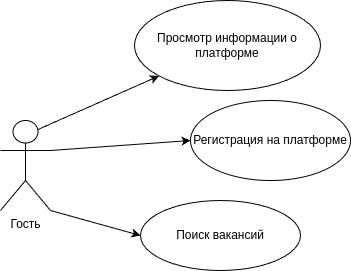
\includegraphics[width=1\linewidth]{p1}
	\caption{Диаграмма прецедентов для категории пользователей - гость}
	\label{p1:image}
\end{figure}

Соискателю должны быть доступны следующие функции:

\begin{enumerate}
	\item Авторизация на платформе.
	\item Создание и редактирование резюме.
	\item Поиск вакансий.
	\item Отклик на вакансию.
\end{enumerate}

Прецеденты для соискателя представлены на рисунке ~\ref{p2:image}.

\begin{figure}[H]
	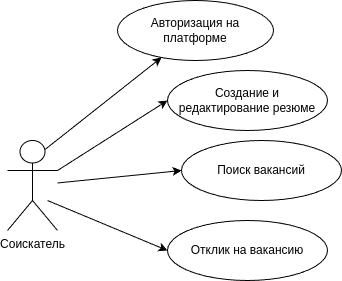
\includegraphics[width=1\linewidth]{p2}
	\caption{Диаграмма прецедентов для категории пользователей - соискатель}
	\label{p2:image}
\end{figure}

Работодателю должны быть доступны следующие функции:

\begin{enumerate}
	\item Авторизация на платформе.
	\item Публикация вакансии.
	\item Просмотр резюме соискателей.
	\item Просмотр откликов на вакансию.
\end{enumerate}

\begin{figure}[H]
	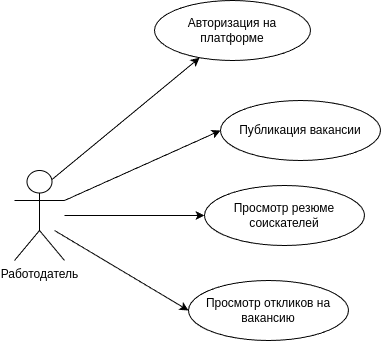
\includegraphics[width=1\linewidth]{p3}
	\caption{Диаграмма прецедентов для категории пользователей - работодатель}
	\label{p3:image}
\end{figure}

Aдминистратору должны быть доступны следующие функции:

\begin{enumerate}
	\item Управление пользователями.
	\item Модерация вакансий и резюме.
	\item Управление информационными разделами.
\end{enumerate}

\begin{figure}[H]
	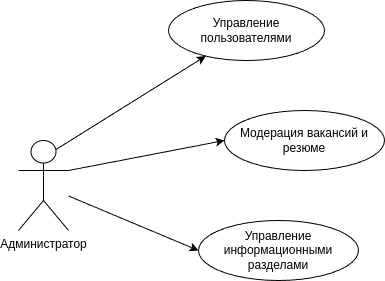
\includegraphics[width=1\linewidth]{p4}
	\caption{Диаграмма прецедентов для категории пользователей - администратор}
	\label{p4:image}
\end{figure}

\subsection{Требования к оформлению документации}

Разработка программной документации и программного изделия должна производиться согласно ГОСТ 19.102-77 и ГОСТ 34.601-90. Единая система программной документации.
